\documentclass[tikz,border=5pt]{standalone}
\usepackage{amsmath, amssymb}
\usetikzlibrary{arrows.meta, calc}

\begin{document}
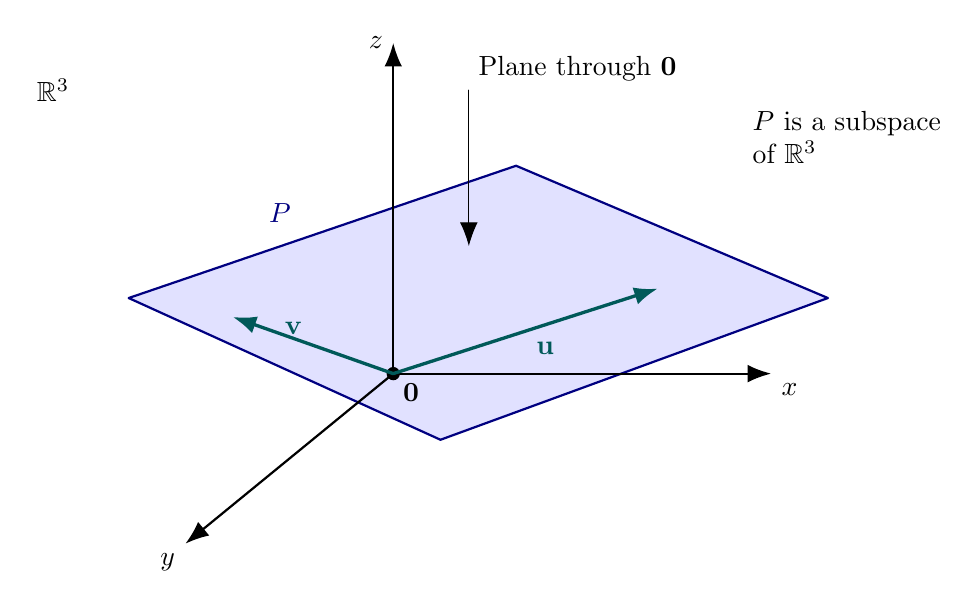
\begin{tikzpicture}[scale=1.2, line cap=round, line join=round]

    % Definición visual de ejes en pseudo-3D
    \coordinate (O) at (0,0);
    \coordinate (X) at (4,0);
    \coordinate (Y) at (-2.2,-1.8);
    \coordinate (Z) at (0,3.5);

    % Plano que pasa por el origen
    \fill[blue!15, opacity=0.8]
        (-2.8,0.8) -- (1.3,2.2) -- (4.6,0.8) -- (0.5,-0.7) -- cycle;

    \draw[thick, blue!50!black]
        (-2.8,0.8) -- (1.3,2.2) -- (4.6,0.8) -- (0.5,-0.7) -- cycle;

    % Ejes
    \draw[-{Latex[length=3mm]}, thick] (O) -- (X) node[below right] {$x$};
    \draw[-{Latex[length=3mm]}, thick] (O) -- (Y) node[below left] {$y$};
    \draw[-{Latex[length=3mm]}, thick] (O) -- (Z) node[left] {$z$};

    % Origen
    \fill (O) circle (2pt);
    \node[below right] at (O) {$\mathbf{0}$};

    % Vectores dentro del plano
    \draw[-{Latex[length=3mm]}, very thick, teal!70!black] (O) -- (2.8,0.9)
        node[midway, below right] {$\mathbf{u}$};

    \draw[-{Latex[length=3mm]}, very thick, teal!70!black] (O) -- (-1.7,0.6)
        node[midway, above left] {$\mathbf{v}$};

    % Etiqueta del plano
    \node[blue!50!black] at (-1.2,1.7) {$P$};

    % Línea vertical para señalar el plano
    \draw[-{Latex[length=3mm]}, thin] (0.8,3.0) -- (0.8,1.35);
    \node[above right] at (0.8,3.0) {Plane through $\mathbf{0}$};

    % Texto explicativo
    \node[align=left] at (4.8,2.5)
    {$P$ is a subspace\\ of $\mathbb{R}^3$};

    % Etiqueta del espacio
    \node at (-3.6,3.0) {$\mathbb{R}^3$};

\end{tikzpicture}
\end{document}